\subsection{Protokolle}
\subsubsection{UART}
\paragraph{Grundlagen}
\subparagraph{Parität}
Das Paritätsbit dient als Ergänzung einer Folge von Bits. Durch das Ergänzen und das entsprechende Setzen des Bits, wird sichergestellt,
dass die Anzahl der Bits gerade ist.

\smallskip

\begin{wrapfigure}{r}{0.3\textwidth}
    % \begin{figure}[h]
     \vspace{-\baselineskip}
         \centering
         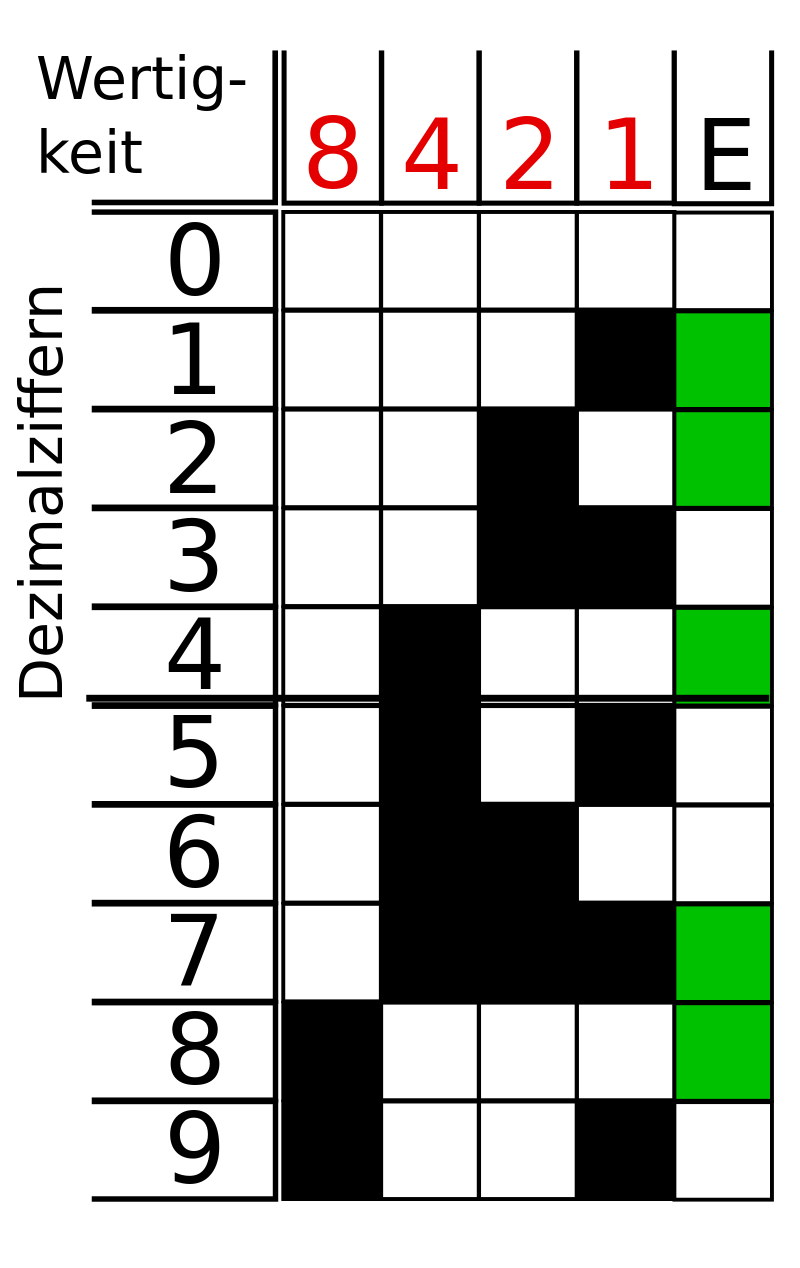
\includegraphics[scale=0.1]{Pictures/paritaet.png}
         \caption{\textit{Parität \citep{ImgParitaet}}}
         \label{img:paritaet}
    % \end{figure}
 \end{wrapfigure}

\smallskip
Die Nutzung eines Paritätsbits ist die einfachste aller Möglichkeiten, Übertragungsfehler zu erkennen. Kippt während der Übertragung eines
der zu übertragenen Bits, ist die Zahl der Bits nicht mehr gerade - ein Fehler liegt vor.

Es ist allerdings nicht möglich festzustellen, wo genau der Fehler aufgetreten ist \citep{Bussysteme}.

\smallskip

Abb. \ref{img:paritaet} zeigt die Applikation eines Paritätsbits bei der binären Repräsentation der Dezimalzahlen eins bis acht. Sobald die Anzahl der 
gesetzten Bits ungerade ist, wird ein Paritätsbit (E) hinzugefügt.

\subparagraph{Baudrate}\label{para:baud}

Die Baudrate, auch Symbolrate genannt, beschreibt die Geschwindigkeit mit der Zeichen übertragen werden.

Ein Baud entspricht hierbei ein Zeichen pro Sekunde \citep{Bussysteme}.

Beispiele für gängige, standarisierte Baudraten für die Übertragung per \ac{UART} sind:

\begin{itemize}
    \item 4800 Baud
    \item 9600 Baud
    \item 115200 Baud
\end{itemize}

Diese Baudraten werden von den meisten Computer- oder Prozessorsystemen unterstützt \citep{Bussysteme}.

\newpage

\paragraph{Erklärung}

Der \acl{UART} ist eine elektronische Schaltung, oder im Falle eines \ac{uC}, eine Peripherieeinheit, welche
die Datenübertragung mit einem anderen System ermöglicht. Die Übertragung läuft hierbei asynchron,
d.h. ohne ein Taktsignal, welches ebenfalls übertragen wird, ab \citep{Bussysteme}. Die Übertragungsgeschwindigkeit
wird in Baud  \ref{para:baud} angegeben.

\smallskip

\begin{wrapfigure}{r}{0.3\textwidth}
    % \begin{figure}[h]
     \vspace{-\baselineskip}
         \centering
         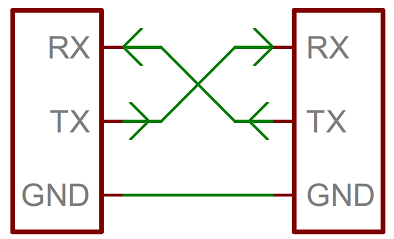
\includegraphics[scale=0.45]{Pictures/uart_rx_tx.png}
         \caption{\textit{Verbindung \citep{ImgRXTX}}}
         \label{img:uart_rxtx}
    % \end{figure}
 \end{wrapfigure}


Jede Seite der Übertragung verfügt über zwei Anschlüsse, \textbf{RX} und \textbf{TX}. \textbf{RX} steht hierbei
für Receiver (\textit{engl. Empfänger}), währen \textbf{TX} für Transmitter (\textit{engl. Sender}) steht.

Für eine korrekte Funktion müssen die beiden Anschlüsse "über Kreuz", wie in Abb. \ref{img:uart_rxtx} dargestellt, verbunden werden \citep{Mikroprozessortechnik}.

\smallskip

Es existieren verschiedene Implementationen von \ac{UART}, welche sich in der Nachrichtenlänge und der Art der
Parität unterscheiden (gerade oder ungerade Parität). Ein oft genutztes Format ist das s.g. \textbf{8N1}-Format.

\smallskip


Die Abkürzung steht hierbei für 8 Bits Nachrichtenlänge und \textit{keine} Parität und ein Stop-Bit. Es wird jedoch neben dem \textit{Stop-}Bit
immer noch ein weiteres Bit übertragen, das \textit{Start-}Bit. Diese zwei Bits repräsentieren das s.g. Framing \textit{engl.: Einrahmen} 
(siehe Abb. \ref{img:uart_framing}) und signalisieren den Beginn und das Ende der Nachricht. Der Beginn einer Nachricht wird mit einem 
Wechsel von '1' auf '0' signalisiert, während das Ende einer Nachricht mit einem Wechsel von '0' auf '1' signalisiert wird \citep{Mikroprozessortechnik}. 

\vspace{0.5cm}

\begin{figure}[h]
    \vspace{-\baselineskip}
        \centering
        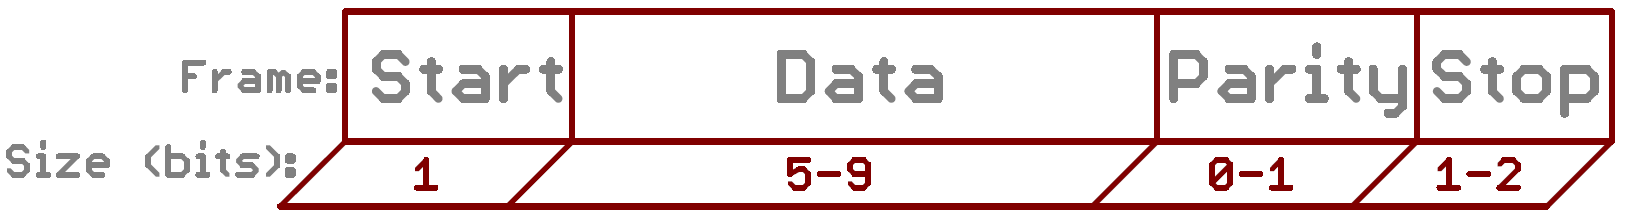
\includegraphics[scale=0.3]{Pictures/uart_framing.png}
        \caption{\textit{Framing \citep{ImgRXTX}}}
        \label{img:uart_framing}
\end{figure}

Sollen nun z.B. die ASCII-Zeichen '\textbf{O}' und '\textbf{K}' im 8N1-Format übertragen werden, 
sähe die Bitreihenfolge wie in Abb. \ref{img:uart_ok} dargestellt aus. Es ist dabei zu beachten, dass das
\acs{LSB} zuerst übertragen wird.

\vspace{0.5cm}

\begin{figure}[h]
    \vspace{-\baselineskip}
        \centering
        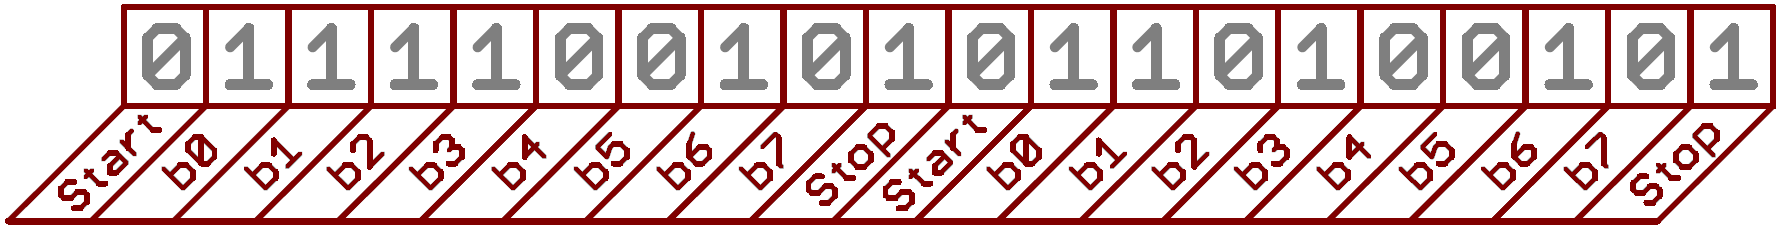
\includegraphics[scale=0.3]{Pictures/uart_ok.png}
        \caption{\textit{Nachricht 'OK' \citep{ImgRXTX}}}
        \label{img:uart_ok}
\end{figure}

Die Bitfolge '01001111' entspricht dem Buchstaben 'O', die Bitfolge '01001011' die dem Buchstaben 'K'.



\subsubsection{MQTT} 

MQTT ist ein simples Client-Server-Protokoll zur Nachrichtenübertragung, häufig genutzt in \ac{IoT}-Anwendungen oder im industriellen Umfeld. Durch
die geringe Belegung von Bandbreite eignet es sich in Netzwerken mit hoher Latenz, schlechten Verbindungen und zur Nutzung auf Geräten
mit vergleichsweise geringer Rechenleistung \citep{MQTT_FAQ}.

\smallskip

Geräte, welche Daten empfangen oder versenden (s.g. Clients) sind mit einem zentralem Server (s.g. Broker) verbunden. Nach erfolgreicher Verbindung
der Clients mit dem Broker versenden diese ihre Nachrichten mit einem s.g. Topic, welches die versendete Nachricht hierarchisch einstuft.
Ein Beispiel wäre zum Beispiel \lstinline!Hochschule/B/Temp!. Sendet nun ein Client eine Nachricht mit diesem Topic, wird 
diese Nachricht an alle Clients weitergeleitet, welche dieses Topic abonniert haben. Diese Art der Kommunikation wird Publish/Subscribe-Modell 
genannt \citep{MQTT_Article} und wird in Abb. \ref{img:MQTT} dargestellt. 

\begin{figure}[h]
    \vspace{-\baselineskip}
        \centering
        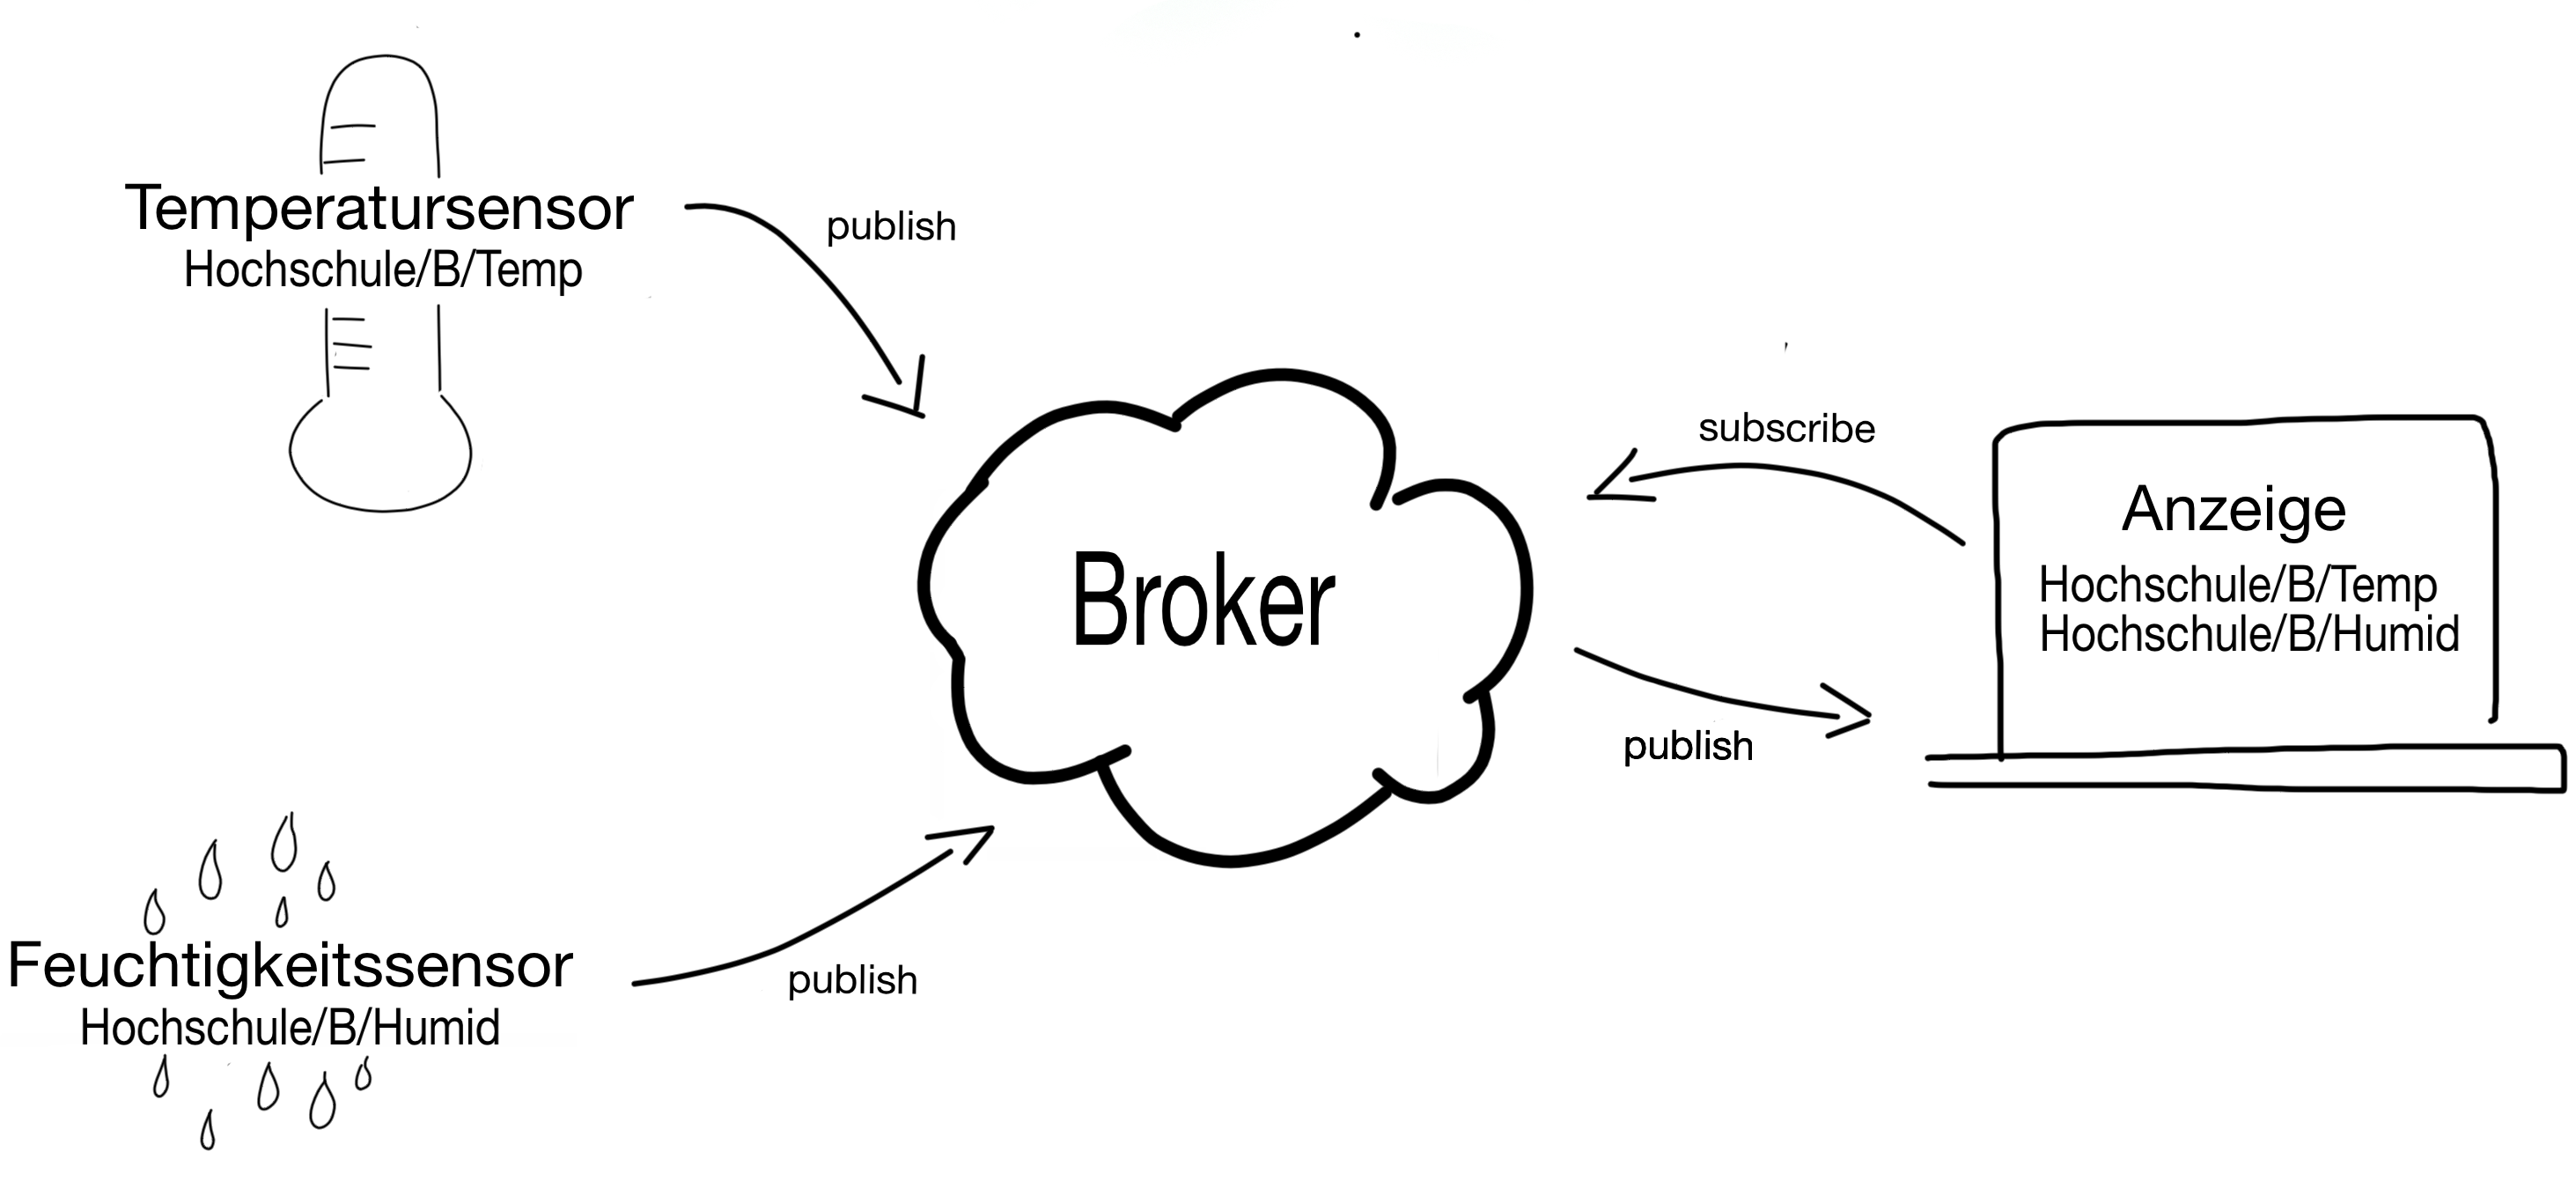
\includegraphics[scale=0.5]{Pictures/brokerclient.png}
        \caption{\textit{Publish/Subscribe-Modell}}
        \label{img:MQTT}
\end{figure}

\smallskip

MQTT besitzt diverse Features, welche, abgesehen von der Simplizität, attraktiv für den Einsatz im industriellen Umfeld sind \citep{MQTT_Article}:

\paragraph{Quality of Service Level}
Durch den Quality of Service Level kann sichergestellt werden, dass eine Nachricht beim Empfänger ankommt, auch wenn es zu Verbindungsabbrüchen kommt.
\paragraph{Retained Messages}
Die letzte gesendete Nachricht eines Topics wird im Broker hinterlegt. Verbindet sich ein neuer Client mit diesem Topic, erhält er automatisch
die gespeicherte Nachricht.
\paragraph{Last Will and Testament}
Sobald der Broker feststellt, dass ein Client die Verbindung ohne eine Abmeldung verloren hat, wird eine Nachricht an alle Clients, welche das
selbe Topic abonniert haben, versendet.
\paragraph{Persistent Sessions}
Falls mit häufigen Verbindungsabbrüchen zu rechnen ist, kann der Broker alle durch einen Verbindungsabbruch verpasste Nachrichten automatisch 
erneut an den Client versenden.


